\section{Ejercicio 1 - TaskConsola}

Se programó un tipo de tarea llamado {\tt TaskConsola}, que se ocupa de realizar {\it n} llamadas bloqueantes, cada una con una duración al azar comprendida entre los valores {\it bmin} y {\it bmax}.

\subsection{Algoritmo}

La Figura \ref{cod-tconsola} muestra el pseudocódigo de esta tarea.

\begin{figure}[!htb]
\begin{codebox}
\Procname{$\proc{TaskConsola}(n,bmin,bmax)$}
\li \For $i \leftarrow 0 .. n$
\li \Do 	$ciclos\_bloqueo \leftarrow$ valor ``random'' en $[bmin,bmax]$
\li 		bloquear durante $ciclos\_bloqueo$ ciclos
\End
\end{codebox}
\caption{Pseudocódigo TaskConsola}\label{cod-tconsola}
\end{figure}

Para el cálculo del valor ``random'' se utilizó la función {\tt rand()} provista por la librería {\tt stdlib} de C++.

\subsection{Pruebas}

Se creó un lote con 3 tareas de tipo {\tt TaskConsola} para correr en el simulador con un scheduler FCFS.  La Figura \ref{fig-1} muestra el resultado de dicha simulación.

\begin{figure}[!htb]
\begin{center}
  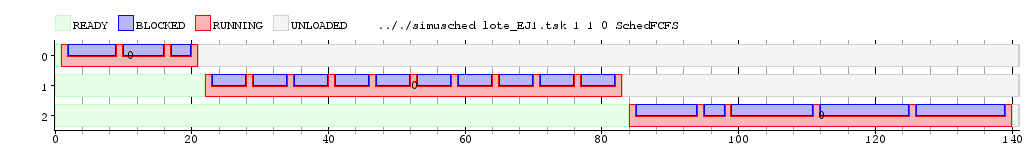
\includegraphics[scale=0.45]{imagenes/ej1.png}
\end{center}
\caption{Simulación lote TaskConsola con FCFS, 1 núcleo, 1 ciclos de cs}\label{fig-1}
\end{figure}